\chapter{Распределенный метод длинных характеристик}

Метод длинных характеристик является наиболее точным методом решения уравнения переноса излучения. Метод основывается на точном решении уравнения переноса в каждом направлении.

Уравнение переноса 
\[
(\vec \Omega \nabla) I(\vec r, \vec \Omega) + \varkappa(\vec r, \vec \Omega) I(\vec r, \vec \Omega) = \varkappa(\vec r, \vec \Omega) I_\text{p}(\vec r, \vec \Omega)
\]
вдоль характеристики
$
\vec r - \vec r_0 = \vec \Omega (s - s_0)
$
превращается в обыкновенное дифференциальное уравнение
\[
\frac{dI(s)}{ds} + \varkappa(s) I(s) = \varkappa(s) I_\text{p}(s)
\]
и может быть легко проинтегрировано точно:
\begin{equation}
I(s) = I(s_0) e^{-\tau(s_0, s)} + \int_{s_0}^s \varkappa(\xi) I_\text{p}(\xi)
e^{-\tau(\xi,s)} d\xi.
\label{eq:exact}
\end{equation}
В последнем выражении $\tau(a,b) = \int_a^b \varkappa(s) ds$ --- оптическая длина отрезка характеристики от точки $s = a$ до точки $s = b$.

Соотношение \eqref{eq:exact} лежит в основе метода длинных характеристик. В отличие от метода коротких характеристик, где характеристика выпускается из узла до входной грани тетраэдра, в методе длинных характеристик она выпускается до границы расчетной области, см. рисунок \ref{fig:lcm}.
\begin{figure}[ht!]
\centering
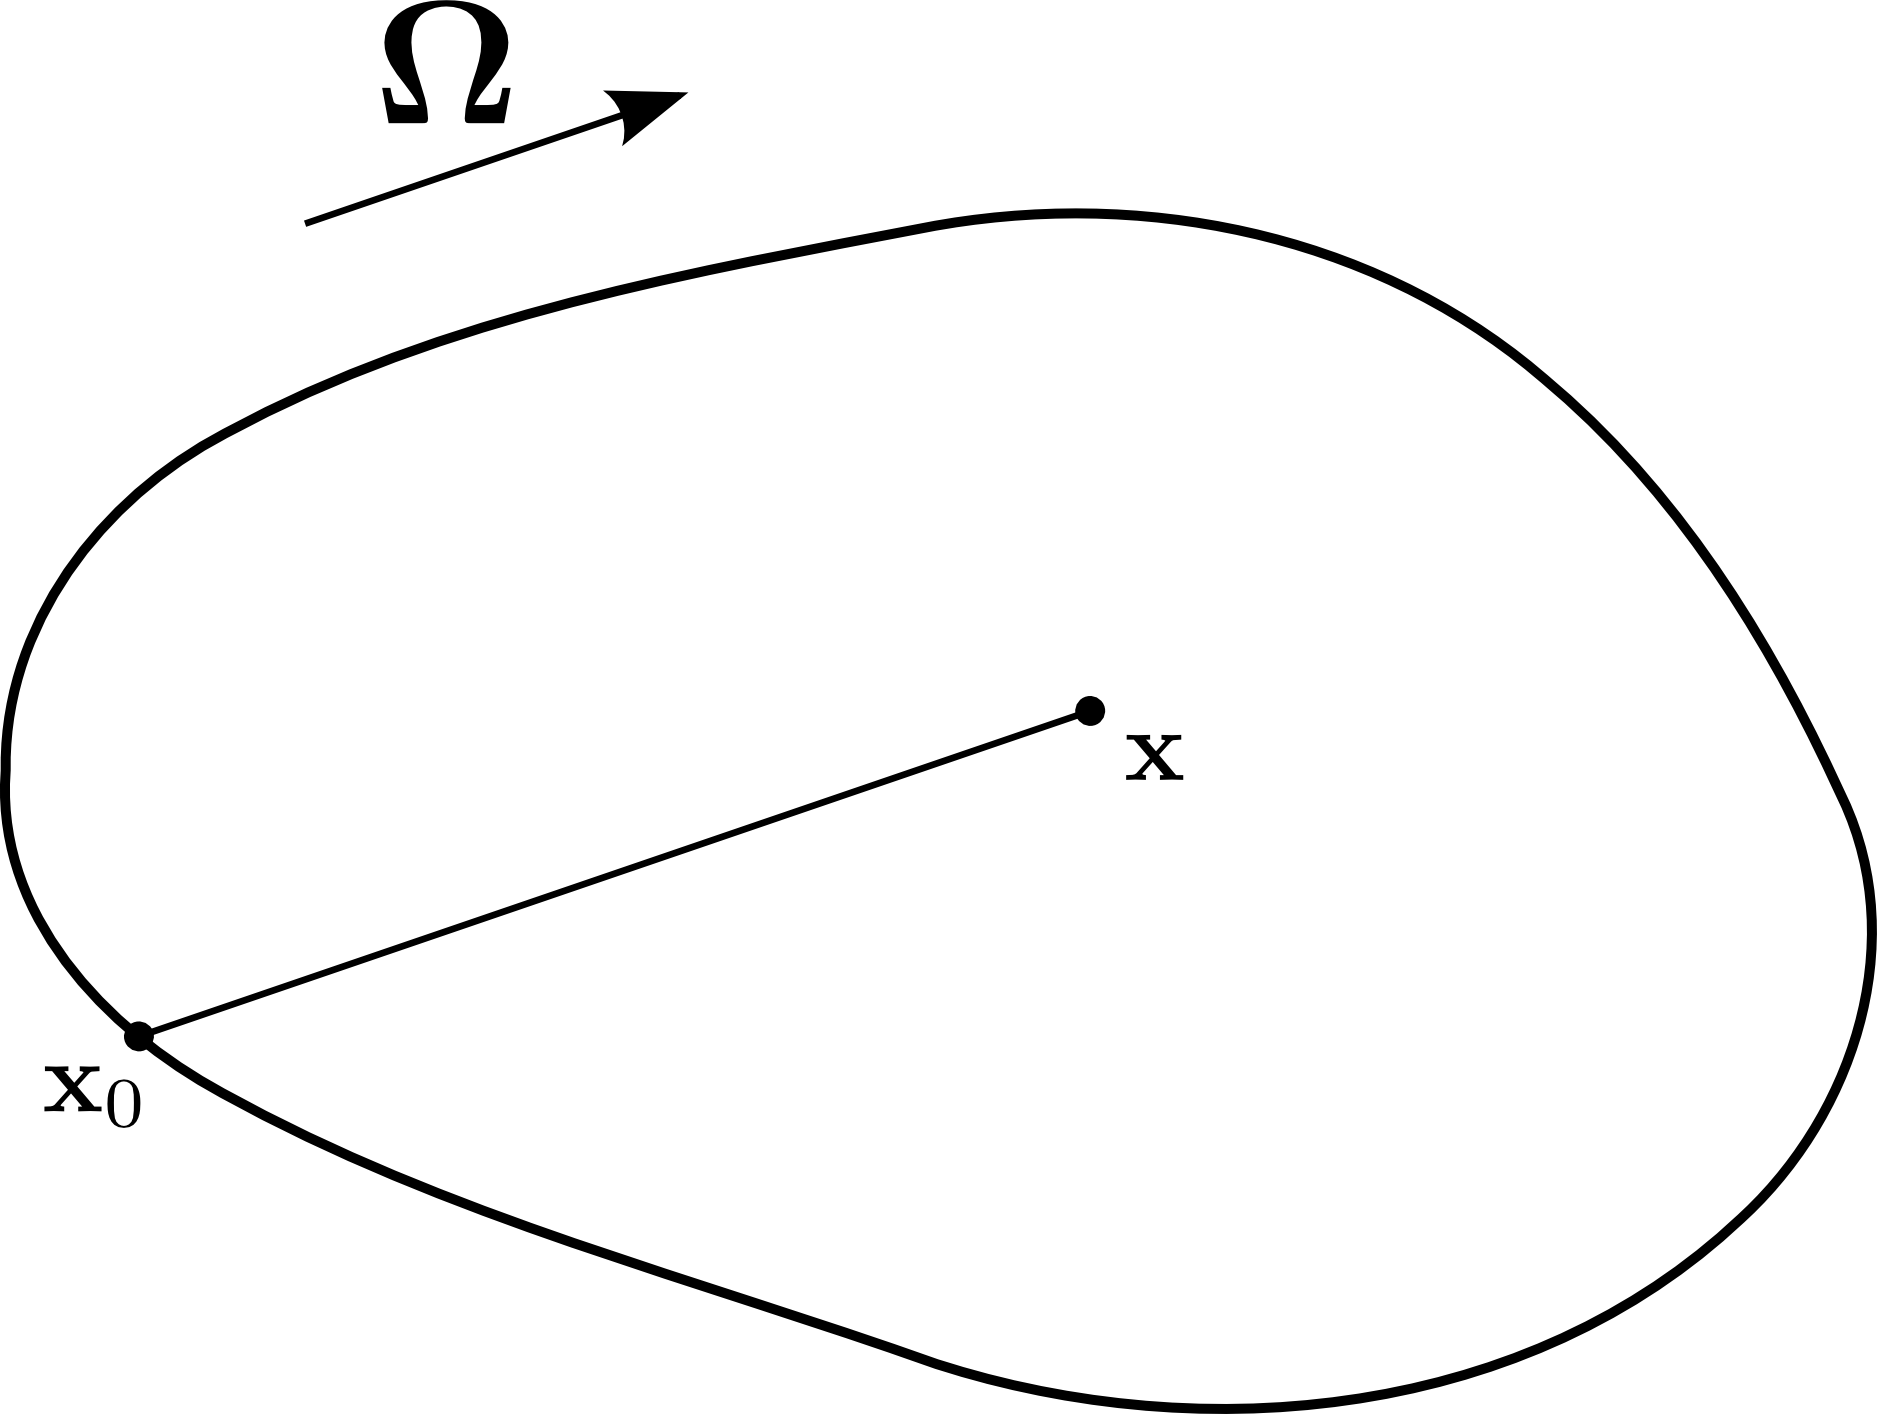
\includegraphics[height=0.25\textheight]{lcm.png}
\caption{Нахождение решения методом длинных характеристик}
\label{fig:lcm}
\end{figure}

\section{Функция Грина для задачи переноса излучения}

Заметим, что соотношение \eqref{eq:exact} представляет собой выражение функции Грина, так как связывает решение в точке $I(\vec r, \vec \Omega)$ с граничным условием $I(\vec r_0, \vec \Omega), \vec r_0 \in \partial G$.

Введем обозначения $\alpha(s_0, s)$ и $\beta(s_0, s)$ 
\begin{gather*}
\alpha(s_0, s) = e^{-\tau(s_0, s)}\\
\beta(s_0, s) = \int\limits_{s_0}^s \varkappa(\xi) I_\text{p}(\xi) \alpha(\xi, s) d\xi.
\end{gather*}

В этих обозначениях функция Грина записывается в виде
\begin{equation}
I(s) = \alpha(s_0, s) I(s_0) + \beta(s_0, s).
\label{eq:connection}
\end{equation}
При $s > s_0$ для величин $\alpha(s_0, s), \beta(s_0, s)$ справедливо
\begin{equation}
\begin{gathered}
0 < \alpha(s_0, s) \leqslant 1\\
0 \leqslant \beta(s_0, s) \leqslant \max_{\xi \in [s_0, s]} I_\text{p}(\xi)
\cdot \int_{s_0}^s \varkappa(\xi) e^{-\tau(\xi, s)} d\xi = \\ =
\max_{\xi \in [s_0, s]} I_\text{p}(\xi)
\cdot \int_{0}^{\tau(s_0,s)} e^{-u} du =
(1 - \alpha(s_0, s))\max_{\xi \in [s_0, s]} I_\text{p}(\xi).
\end{gathered}
\label{eq:limits}
\end{equation}
С учетом \eqref{eq:limits} для $I(s)$ верен принцип максимума
\[
I(s) \leqslant \alpha(s_0, s) I(s_0) + (1 - \alpha(s_0, s))\max_{\xi \in [s_0, s]} I_\text{p}(\xi) \leqslant \max\left(I(s_0); \max_{\xi \in [s_0, s]} I_\text{p}(\xi)\right).
\]

Фактически, функция Грина задается лишь двумя коэффициентами для каждой точки $\vec r$ и направления $\vec \Omega$. В численном методе точка $\vec r_0$ не является узлом сетки, а значение $I(\vec r_0, \vec \Omega)$ находится интерполяцией интенсивности по грани, содержащей точку $\vec r_0$. При этом численная функция Грина дополнительно задается коэффициентами интерполяции и номерами вершин грани.

Для сравнения, численная функция Грина, построенная в методе коротких характеристик, зависит от большого числа узлов на границе. Увеличение шаблона вызвано в этом методе многократной интерполяцией.

\subsection{Трассировочное соотношение}

Для практического вычисления коэффициентов $\alpha(s_0, s)$ и $\beta(s_0, s)$ удобно пользоваться следующим соотношением при $s_0 \leq s_1 \leq s$:
\[
\alpha(s_0, s) = e^{-\tau(s_0, s)} = 
e^{-\tau(s_0, s_1) -\tau(s_1, s)} = 
\alpha(s_0, s_1)\alpha(s_1, s),
\]
следующим из аддитивности оптической длины.

Для $\beta(s_0, s)$ справедливо
\begin{multline*}
\beta(s_0, s) = 
\int\limits_{s_0}^s \varkappa(\xi) I_\text{p}(\xi) \alpha(\xi, s) d\xi = \\ =
\int\limits_{s_0}^{s_1} \varkappa(\xi) I_\text{p}(\xi) \alpha(\xi, s) d\xi +
\int\limits_{s_1}^s \varkappa(\xi) I_\text{p}(\xi) \alpha(\xi, s) d\xi = \\ =
\int\limits_{s_0}^{s_1} \varkappa(\xi) I_\text{p}(\xi) \alpha(\xi, s_1) \alpha(s_1, s) d\xi +
\int\limits_{s_1}^s \varkappa(\xi) I_\text{p}(\xi) \alpha(\xi, s) d\xi = \\
= \beta(s_0, s_1) \alpha(s_1, s) + \beta(s_1, s).
\end{multline*}

Фактически, соотношения между коэффициентами $\alpha, \beta$ следуют из принципа Гюйгенса
\begin{multline*}
I(s) = \alpha(s_1, s) I(s_1) + \beta(s_1, s) = \\ =
\alpha(s_1, s) \Big(\alpha(s_0, s_1) I(s_0) + \beta(s_0, s_1)\Big) + \beta(s_1, s)
= \\ =
\alpha(s_0, s_1)\alpha(s_1, s) I(s_0) + \beta(s_0, s_1)\alpha(s_1, s) + \beta(s_1, s).
\end{multline*}

Будем называть соотношения
\begin{equation}
\begin{gathered}
\alpha(s_0, s) = \alpha(s_0, s_1)\alpha(s_1, s),\\
\beta(s_0, s) = \beta(s_0, s_1) \alpha(s_1, s) + \beta(s_1, s)
\end{gathered}
\end{equation}
трассировочными. С помощью них удобно вычислять коэффициенты $\alpha(s_0, s), \beta(s_0, s)$, двигаясь вдоль характеристики по тетраэдрам триангуляции (см. рисунок \ref{fig:trace}). При переходе от коэффициентов $\alpha(s_1, s), \beta(s_1, s)$ к коэффициентам $\alpha(s_0, s), \beta(s_0, s)$ достаточно знать только значения
$\alpha(s_0, s_1), \beta(s_0, s_1)$. Для однородных значений $\varkappa, I_\text{p}$ в тетраэдре,
\[
\alpha(s_0, s_1) = e^{-\varkappa (s_1 - s_0)},\qquad
\beta(s_0, s_1) = \big(1 - \alpha(s_0, s_1)\big) I_\text{p}.
\]
\begin{figure}[ht!]
\centering
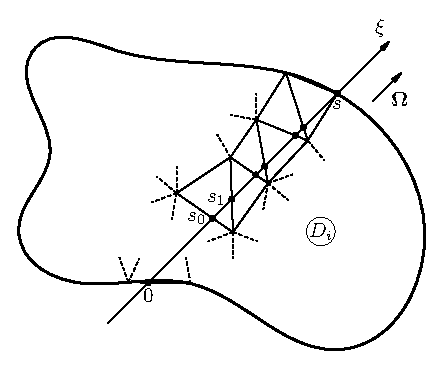
\includegraphics[width=.4\textwidth]{trace-0.eps}
\caption{Трассировка луча по триангуляции}
\label{fig:trace}
\end{figure}

\section{Устойчивая трассировки луча}

Рассмотрим процесс трассировки луча из точки $\vec r$. Трассировка начинается в тетраэдре $T$, содержащем точку $\vec r - 0 \vec \Omega$. Для каждой треугольной грани $Q = \operatorname{conv}(r_1, r_2, r_3)$ тетраэдра находятся барицентрические координаты $\gamma_k$ точки пересечения $\vec r^* = \sum_{k=1}^3 \gamma_k \vec r_k$ плоскости грани с лучом $\vec r - \vec \Omega s$.  Находится грань, для которой все барицентрические координаты $\gamma_k$ неотрицательны. Для этой грани $\vec r^* \in Q$. Псевдокод данной процедуры изложен в алгоритме \ref{alg:traceelem}  
\begin{algorithm}[ht!]
\centering
\begin{algorithmic}[1]
\Function{TraceElement}{$e$, $P \in e, \vec \omega$}
%\State $P := $ \Call{ShiftToStable}{$e, P$}
\For{каждой грани $f \in e$}
\State $(\vec r_1, \vec r_2, \vec r_3) := $ \Call{VertexCoordinates}{$f$}
\State $\triangleright$  Решить
$(
\vec r_P - \ell \vec \omega - \vec r_1,
\vec r_2 - \vec r_1,
\vec r_3 - \vec r_1
) = 0$ относительно $\ell$
\If{$(\vec \omega, \vec r_2 - \vec r_1, \vec r_3 - \vec r_1) = 0$}
\State $\mu(f) := \infty$
\State \textbf{continue} \Comment Перейти к следующей грани
\EndIf
\State $\ell := 
\dfrac{(\vec r_P - \vec r_1, \vec r_2 - \vec r_1, \vec r_3 - \vec r_1)}
{(\vec \omega, \vec r_2 - \vec r_1, \vec r_3 - \vec r_1)}$
\If{$\ell < 0$}
\State $\mu(f) := \infty$
\State \textbf{continue} \Comment Перейти к следующей грани
\EndIf
\State $\vec r_Q := \vec r_P - \ell \vec \omega$
\State $\vec\gamma(f) = $ \Call{BarycentricCoordinates}{$f, Q$}
\State $\mu(f) := \sum_{k}|\gamma_k(f)|$
\State $\pi(f) := Q$
\EndFor
\State $f := \operatorname{argmin} \mu(f)$
\State\Return{$\pi(f), f, (\vec\omega, \vec r_Q - \vec r_P), \vec \gamma(f)$}
\EndFunction
\end{algorithmic}
\caption{Алгоритм трассировки в элементе}
\label{alg:traceelem}
\end{algorithm}

После прохождения лучом точки $\vec r^*$, трассируемый луч переходит в точку $\vec r^*$ и в тетраэдр $T'$, граничащий с $T$ по грани $Q = T \cap T'$.  Трассировка заканчивается, когда грань $Q$ очередного тетраэдра является граничной.

Параллельно с трассировкой тетраэдров производится вычисление $\alpha(s_0, s), \beta(s_0, s)$. В начале трассировке величины $\alpha, \beta$ инициализируются значениями $\alpha = 1, \beta = 0$.
При прохождении очередного тетраэдра, вычисляются коэффициенты $\tilde \alpha = \alpha(s_0, s_1)$ и $\tilde \beta = \beta(s_0, s_1)$ и производится обновление по правилу
\[\begin{aligned}
\beta &:= \beta + \tilde \beta \alpha\\
\alpha &:= \alpha \tilde \alpha.
\end{aligned}
\]
При завершении трассировки луча переменные $\alpha, \beta$ содержат значения $\alpha(0, s)$ и $\beta(0, s)$.

При практической реализации алгоритма \ref{alg:traceelem} возникает проблема, вызванная ошибками округления. Трассировка может зациклиться, если луч проходит вблизи ребра или вершины.

Введем определения входной и выходной грани, устойчивые к ошибках округлений.
Если $\mathbf n$ --- нормаль к грани, а $\boldsymbol \Omega$ --- направление излучения, то в случае
%\newpage
\begin{itemize}
\item если $(\mathbf n \boldsymbol \Omega) < -\epsilon$, то грань называется входной (луч входит в тетраэдр);
\item если $(\mathbf n \boldsymbol \Omega) > \phantom{-}\epsilon$, то грань называется выходной (луч выходит из тетраэдра);
\item иначе, грань называется касательной.
\end{itemize}
В этом определении $\epsilon \ll 1$ --- малое число. В реализации использовалось $\epsilon = 10^{-6}$.

Рассмотрим выпуклый многогранник $P_1P_2\dots P_n$ и точку $Q$ внутри него. Выпустим из точки $Q$ 
луч в направлении $-\vec\omega$. Этот луч выйдет через некоторую грань $f$ многогранника $T$.

Чтобы луч не выходил через касательную грань достаточно сместить точку $Q$ внутрь многогранника 
$T$. Справедлива следующая лемма:
\newtheorem{lemma}{Лемма}
\begin{lemma}[Об устойчивой трассировке]
Если точка $Q$ в многограннике $T = P_1P_2\dots P_n$ находится на расстоянии более $\delta 
\equiv \epsilon \cdot d(T)$ от каждой грани, то луч из точки $Q$ в направлении
$-\boldsymbol \omega$ выйдет через входную грань многогранника. Здесь $d(T)$ --- диаметр 
многогранника $T$, то есть максимальное расстояние между двумя его точками.
\end{lemma}
\begin{proof}[Доказательство]
Пусть $S$ --- точка грани $f$ многогранника (см. рисунок \ref{fig:touch}), через которую луч выходит из него.
\begin{figure}[ht!]
\centering
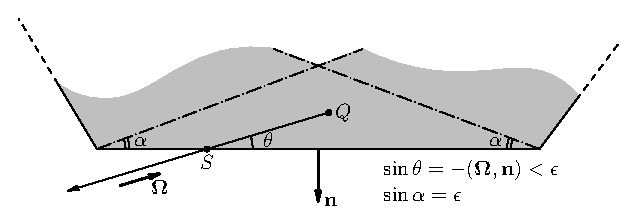
\includegraphics[width=.8\textwidth]{shift-0}
\caption{Точка $Q$ и выходящий из нее касательный луч. Точка $Q$ необходимо должна принадлежать 
серой области}
\label{fig:touch}
\end{figure}

Предположим, что грань является касательной к лучу. Это означает, что $\sin \theta = -(\vec \omega, 
\vec n) \leqslant \epsilon$. Поскольку обе точки $S,Q$ принадлежат $T$, то $|SQ| \leq d(T)$. 
Следовательно, высота, опущенная из $Q$ на грань $f$ не может иметь длину более $\sin \theta \cdot 
d(T) \leq \epsilon \cdot d(T) \equiv \delta$. Следовательно условие $\rho(Q, f) > \delta$ 
гарантирует, что луч не может выйти через грань $f$ так, чтобы быть к ней касательным. Обобщая это 
на все грани многогранника $T$, получаем утверждение леммы.
\end{proof}

Условие данной леммы можно усилить: $\rho(Q, f) > \delta$ является достаточным, но не необходимым. 
Однако, удовлетворить этому условию намного проще, чем точному условию (на рисунке
\ref{fig:forb} точное запрещенное множество закрашено серым цветом, а пунктиром обозначено множество из леммы).
\begin{figure}[ht!]
\centering
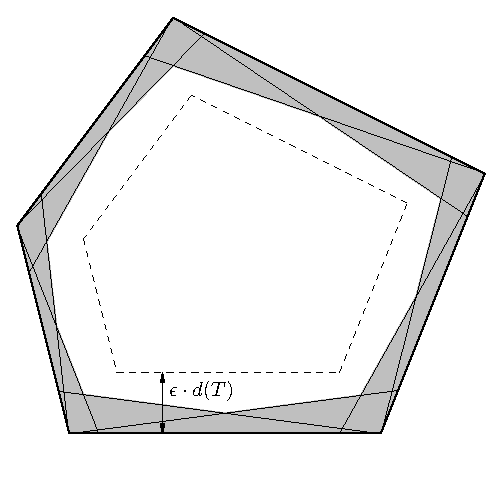
\includegraphics[width=.5\textwidth]{shift-1}%
\caption{Исходный многогранник, запрещенная область (серая) и область из леммы. Для трехмерного 
случая реальная запрещенная область имеет достаточно сложную форму}
\label{fig:forb}
\end{figure}

\begin{figure}[ht!]
\centering
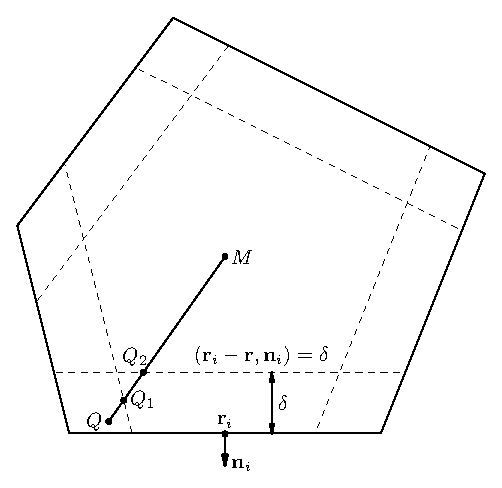
\includegraphics[width=.5\textwidth]{shift-2}%
\caption{Иллюстрация процедуры сдвига точки $Q$ в допустимое множество из леммы}
\end{figure}
Однако, простота этого условия порождает простую процедуру сдвига точки в допустимое множество (при 
условии, что центр масс $M$ многогранника сам лежит в допустимом множестве). Рассмотрим отрезок, 
соединяющий точки $M$ и $Q$, а также все плоскости, содержащие грани многогранника. Пусть каждая из 
этих плоскостей задана уравнением $(\vec r_i - \vec r, \vec n_i) = 0$. Несложно заметить, что 
условия леммы требуют выполнения соотношений $(\vec r_i - \vec r_Q, \vec n_i) > \delta$ для каждой 
$i$-й грани многогранника. Дополнительно требуя, чтобы новая точка $Q_i$ лежала на отрезке $QM$, 
получаем соотношения
\begin{gather*}
\vec r_{Q'} = \lambda \vec r_{Q} + (1 - \lambda) \vec r_{M}, \quad \lambda \in [0,1]\\
\lambda \rightarrow \max_{(\vec r_i - \vec r_{Q_i}, \vec n_i) > \delta}
\end{gather*}
Данная система линейных неравенств на $\lambda$ может быть легко решена последовательно для каждой грани, с выбором минимального $\lambda = \min_i \lambda_i$, см. алгоритм \ref{alg:shift}.

\begin{algorithm}[ht!]
\centering
\begin{algorithmic}[1]
\Function{ShiftToStable}{$e, Q$}
\State $\lambda := 1$
\State $\delta := \epsilon \cdot d(e)$
\State $\vec r_M := $ \Call{MassCenter}{$e$}
\For{каждой грани $f \in e$}
\State $(\vec r_i, \dots) := $ \Call{VertexCoordinates}{$f$}
\Comment Выбрать точку $\vec r_i \in f$
\State $\vec n_i := $ \Call{FaceNormal}{$f$}
\State $\vec r_{Q'} = \lambda \vec r_Q + (1 - \lambda) \vec r_{M}$
\If{$(\vec r_i - \vec r_{Q'}, \vec n_i) > \delta$}
\State \textbf{continue} \Comment Перейти к следующей грани
\Else
\State $\triangleright$ Найти точку пересечения отрезка $QM$ и плоскости
\State $\lambda := \frac{\delta - (\vec r_i - \vec r_M, \vec n_i)}
{(\vec r_Q - \vec r_M, \vec n_i)}$
\EndIf
\EndFor
\State $\vec r_{Q'} = \lambda \vec r_Q + (1 - \lambda) \vec r_{M}$
\State\Return{$Q'$}
\EndFunction
\end{algorithmic}
\caption{Алгоритм смещения точки в элементе}
\label{alg:shift}
\end{algorithm}

Заметим, что при использовании сдвига, длина отрезка характеристики в многограннике не меньше $\delta$, а следовательно при прохождении очередного тетраэдра точка продвигается в направлении $-\vec \Omega$ хотя бы на расстояние $\delta$.
Трассировка области с вычислением коэффициентов $\alpha, \beta$ представлена в алгоритме \ref{alg:tracedom}.

\begin{algorithm}[ht!]
\centering
\begin{algorithmic}[1]
\Function{TraceDomain}{$\mathcal{T}, P \in D, \vec\omega$}
\State $\alpha := 1$
\State $\beta := 0$
\State $e := $ \Call{ContainingElement}{$\mathcal{T}, P$}
\Repeat
\State $(Q, f. \ell, \vec\gamma) :=$ \Call{TraceElement}{$e, P, \vec \omega$}
\State $\Delta := \ell \varkappa(e) $
\Comment{Оптическая толщина элемента $e$}
\State $q := e^{-\Delta}$
\State $\beta := \beta + (1 - q)\alpha I_e(e)$
\State $\alpha := q\alpha$
\State $e := $ \Call{NeighbourOverFace}{$\mathcal{T}, e, f$}
\State $P := Q$
\Until{\textbf{not} \Call{IsValidElement}{$e$}}
\State\Return{$\alpha, \beta, \vec \gamma, f$}
\EndFunction
\end{algorithmic}
\caption{Алгоритм трассировки в триангуляции $\mathcal{T}$ области}
\label{alg:tracedom}
\end{algorithm}

\section{Распределенный метод}

Реализация метода длинных характеристик осложняется, если вычислительная область разбита на подобласти. Обычно каждая подобласть принадлежит своему вычислительному процессу и трассировка характеристики становится сложной коллективной операцией.

Заметим, что формула \eqref{eq:connection} позволяет не только вычислить неизвестное значение $I(s)$ через известное значение $I(s_0)$, но и просто связать
линейным соотношением два значения интенсивности в двух точках на одном луче.
Если интенсивность излучения каким-то образом оказалась известной на границе вычислительных подобластей, то трассировку лучей достаточно провести в каждой подобласти независимо от других. В этом случае точка $\vec r_0$ --- это точка, в которой характеристика пересекает границу \emph{подобласти}, а не всей вычислительной области (см. рис. \ref{fig:mcm}).

\begin{figure}[ht]
\centering
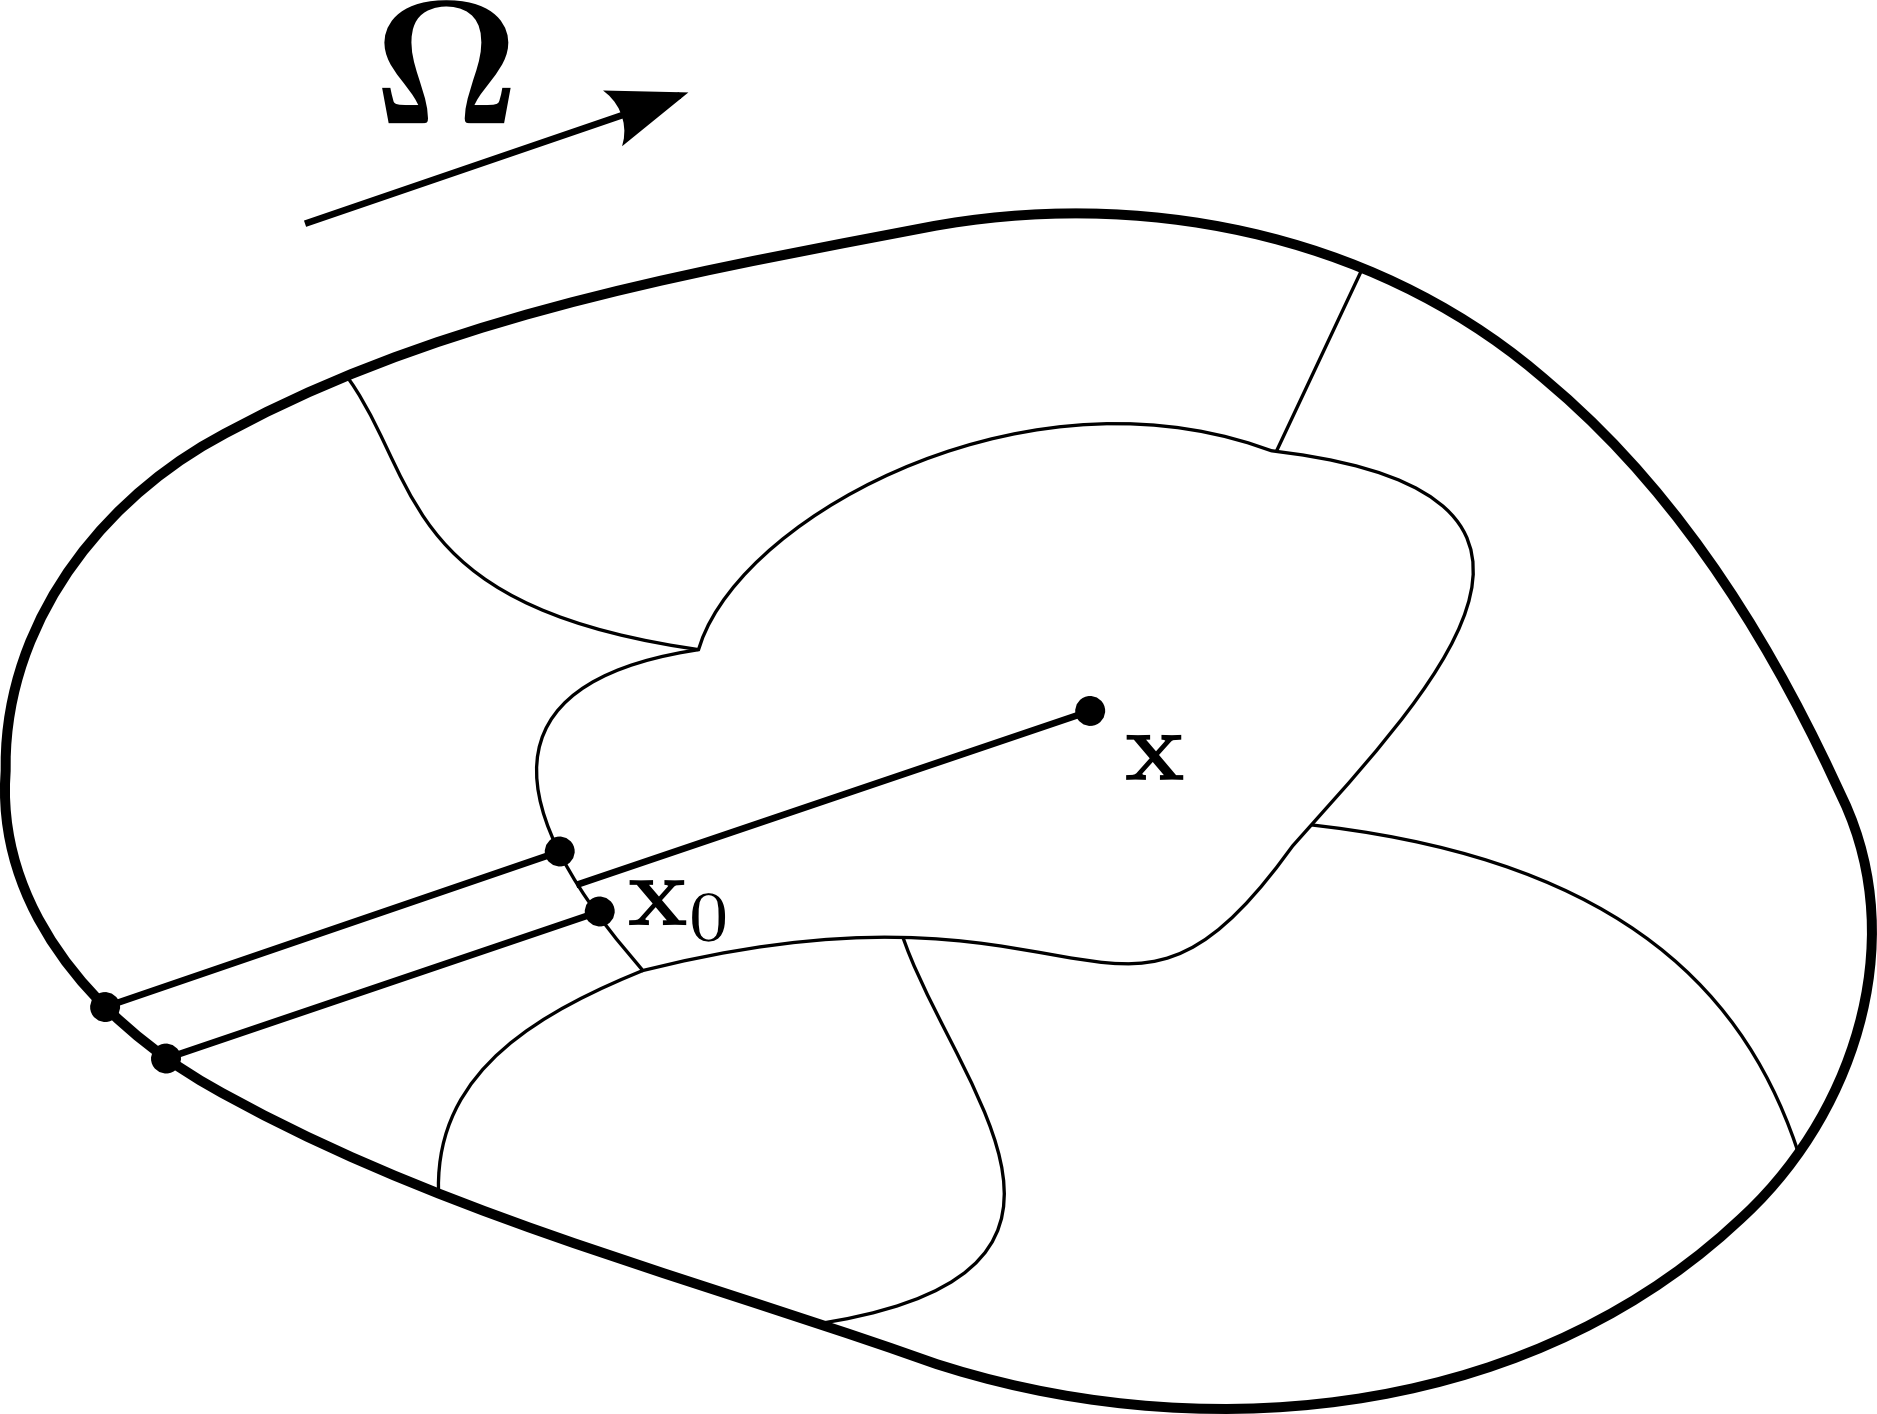
\includegraphics[height=0.3\textheight]{mcm.png}
\caption{Трассировка луча до границы подобласти}
\label{fig:mcm}
\end{figure}

Предположим, что границы подобластей проходят по граням тэтраэдральной сетки, построенной в области. Зафиксируем направление $\vec \Omega$. Будем говорить, что узел сетки (вершина тетраэдра) c координатой $\vec r$ принадлежит подобласти, если точка $\vec r - 0 \vec\Omega$ лежит в подобласти. Если таких подобластей несколько, например, если вектор $\vec \Omega$ лежит в плоскости грани, разделяющей подобласти, выберем подобласть с минимальным номером. Заметим, что определенное таким образом отношение принадлежности зависит не только от геометрических параметров сетки, но и от направления $\vec \Omega$ также. Если узел не принадлежит ни одной подобласти, будем говорить, что он принадлежит \emph{внешней} подобласти, то есть $\mathbb R^3 \setminus G$. Заметим, что интенсивность в граничных узлах, принадлежащих внешней подобласти задана граничными условиями.

Для каждого граничного узла с координатой $\vec r$, принадлежащего подобласти $D_i \subset G$ выпустим характеристику до пересечения с границей подобласти $\partial D_i$. В общем случае, характеристика выйдет из области через некоторую грань $f$ в точке $\vec r_0 = \vec r - \vec \Omega s$. 
Тогда пользуясь соотношением \eqref{eq:connection} заключаем, что
\[
I(\vec r) = \alpha(0, s) I(\vec r_0) + \beta(0, s).
\]
Однако, точка $\vec r$ является узлом расчетной сетки, а точка $\vec r_0$ в общем случае --- нет. Вычислим $I(\vec r_0)$ приближенно интерполяцией интенсивности по вершинам грани $f$
\[
I(\vec r_0) \approx \sum_{j=1}^F \gamma_j I(\vec r_j),
\]
где $F$ --- число вершин грани $f$ (для тетраэдральных сеток $F = 3$), а $\vec r_j$ --- координаты вершин этой грани, которые, в отличие от $\vec r_0$, являются узлами вычислительной сетки. Величины $\gamma_j$ являются обобщенными (для $F > 3$) барицентрическими координатами точки $\vec r_0$ в грани $f$. При этом $\sum_{j=1}^F \gamma_j = 1$.

Таким образом, получается система линейных уравнений, в которые входят значения интенсивности только на границах подобластей, и не входят значения внутри подобластей. Уравнения записаны для каждого граничного узла, принадлежащего некоторой вычислительной подобласти. В узлах, принадлежащих внешней подобласти интенсивность уже задана граничными условиями.

Отметим, что данная система уравнений имеет вид
\begin{equation}
I(\vec r) - \sum_{j=1}^K \gamma_j \alpha(0, s) I(\vec r_j) = \beta(0, s)
\label{eq:slae}
\end{equation}
и имеет диагональное преобладание, поскольку на диагонали стоит коэффициент $1$, а сумма модулей внедиагональных коэффициентов не превосходит $1 - \alpha(0, s) < 1$ некоторые из неизвестных $I(\vec r_j)$ могли быть исключены, если в $\vec r_j$ задано граничное условие).

После коллективного решения системы в узлах на границах подобластей становится известными значения интенсивности. Далее, выпуская характеристики из внутренних точек подобластей восстанавливается решение в каждом узле каждой подобласти всей расчетной области. Эта операция не является коллективной и проводится автономно в каждой подобласти. Также она является самой трудоемкой.

Необходимо подчеркнуть, что решение, полученное данным методом отличается от решения, полученного методом длинных характеристик. В частности, решение зависит от способа декомпозиции на подобласти. Предельный случай декомпозиции области на одну подобласть соответствует методу длинных характеристик, а гипотетический случай декомпозиции на отдельные тетраэдры приводит к методу, где характеристика выпускается от одной грани \emph{тетраэдра} до другой его грани, то есть интерполяция производится на каждой грани, а не только на границе подобласти, как в предлагаемом методе. При этом метод вырождается в метод коротких характеристик. Увеличение количества областей приводит к более частой интерполяции, которая, в свою очередь, вызывает численную диффузию луча. С другой стороны, при этом средняя длина трассируемых лучей уменьшается, что существенно снижает время работы алгоритма.

\section{Параллельная реализация вычислительного алгоритма}

Уравнение переноса решается в некотором наборе направлений. В качестве такого набора были выбраны узлы $\boldsymbol{\omega}_k$ квадратурной формулы для сферы Лебедева 

Для каждого направления $\vec \Omega$ граничные узлы каждой вычислительной подобласти разбиваются на те, которые ей принадлежат (в смысле определения, данного выше) и которые не принадлежат. Из тех, что принадлежат производится трассировка лучей вдоль направления $-\vec \Omega$ до пересечения с границей подобласти алгоритмом \ref{alg:tracedom}.

Таким образом, на каждый процесс формирует в своей подобласти часть общей системы уравнений, в которые входят неизвестные значения интенсивности на границе подобласти.
Далее эта система собирается воедино на одном из процессов, где решается прямым методом для разреженных матриц. Выбор такого метода вместо итерационного обусловлен двумя факторами. Во-первых, размер системы существенно меньше общего количества узлов сетки, так как неизвестные находятся лишь на границах подобластей. Во-вторых, матрицу системы можно превратить в близкую к треугольной, если упорядочить неизвестные по значению их проекции на луч $\vec \Omega$.

Чтобы эффективно использовать остальные процессы, пока на одном из них происходит решение системы, направления обрабатываются не по одному, а по несколько за раз. Это позволяет загрузить все процессы решением систем линейных уравнений, причем каждый процесс будет решать систему для своего направления.

Алгоритм решения состоит из следующих этапов:
\begin{enumerate}
\item Выбирается очередной набор направлений по одному на процесс.
\item Каждый процесс определяет принадлежащие ему точки и производит трассировку от границ в каждом направлении из набора.
\item На каждом процессе собирается система уравнений для его направления из набора.
\item Система решается на каждом процессе и полученное решение рассылается по всем процессам. После этого на каждом процессе становятся известны значения интенсивности на границе его подобласти.
\item В каждой подобласти производится вычисление решения во всех внутренних узлах автономно от остальных процессов.
\item Если остались направления, в которых решение еще не строилось, алгоритм повторяется с первого пункта.
\end{enumerate}

Так как пятый этап алгоритма самый трудоемкий, он был реализован с использованием графических ускорителей. Это позволило не только сократить время расчета задачи, но и произвести перекрытие подготовительных этапов (2-4), производимых на центральном процессоре с этапом 5, производимым на графическом ускорителе (см. рис. \ref{fig:timeline})
\begin{figure}[ht!]
\centering
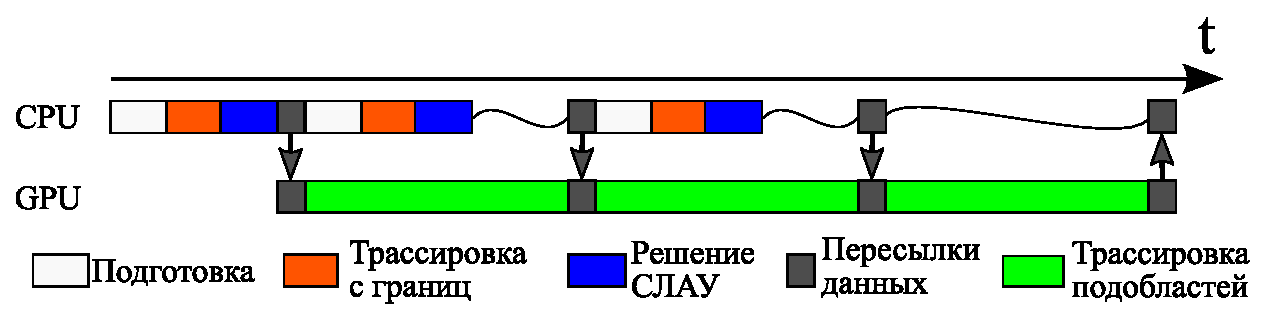
\includegraphics[width=0.8\linewidth]{timeline.eps}
\caption{Временная развертка алгоритма}
\label{fig:timeline}
\end{figure}
